\begin{frame}{Das dritte Graphenmodell}
	\framesubtitle{Es ist das dritte Graphenmodell mit einem Klappstuhl?!?!!}
	
	\begin{itemize}
		\item In MOTIS gibt es noch ein drittes großes Graphenmodell: Den \textbf{Abhängigkeitsgraphen}
		\item Abhängigkeiten zwischen Zügen und Stationen
		\item Wichtig für \textbf{Verspätungen}!
	\end{itemize}

	\begin{center}
		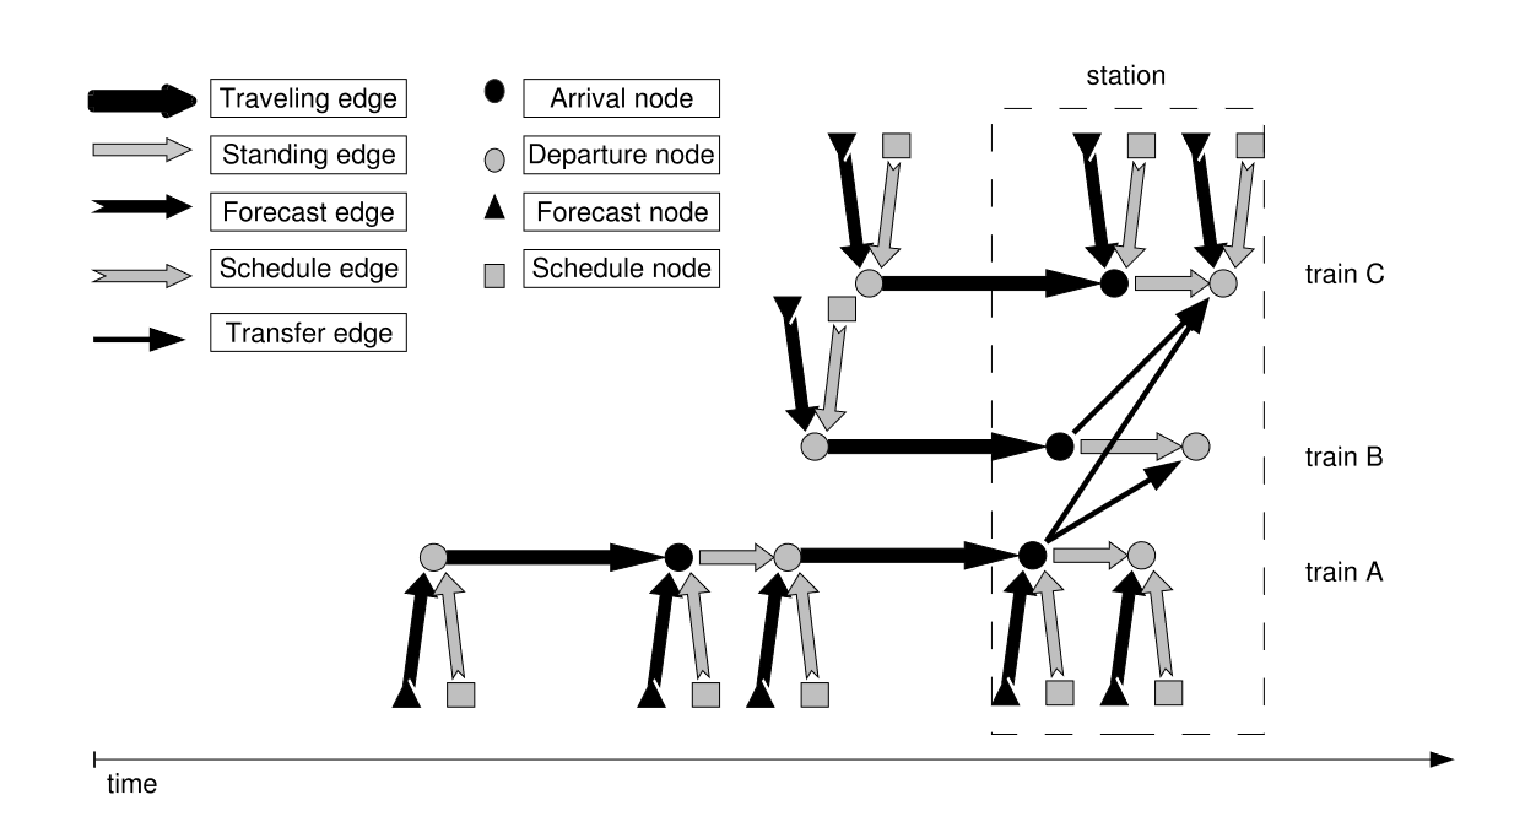
\includegraphics[height=4cm]{images/dependency/dependency-graph.pdf} 
	\end{center}
\end{frame}


\begin{frame}{Zusammenfassung}
	\framesubtitle{Sachen zum Mitnehmen für die späteren Vorträge...}
	\begin{itemize}
		\item Time-Expanded vs. Time-Dependent
		\begin{itemize}
			\item Umstiegszeiten, Fußwege, Takt
			\item In MOTIS: Time-Expanded
		\end{itemize}
		\item Größenordnungen der Graphen unterscheiden sich stark
		\item Für realistische Anwendung: Jeweils unterschiedliche Verfeinerungen und Anpassungen notwendig
	\end{itemize}

\end{frame}

\begin{frame}{Time-Expanded}
	\framesubtitle{Nochmal zum Mitnehmen}
	\begin{center}
		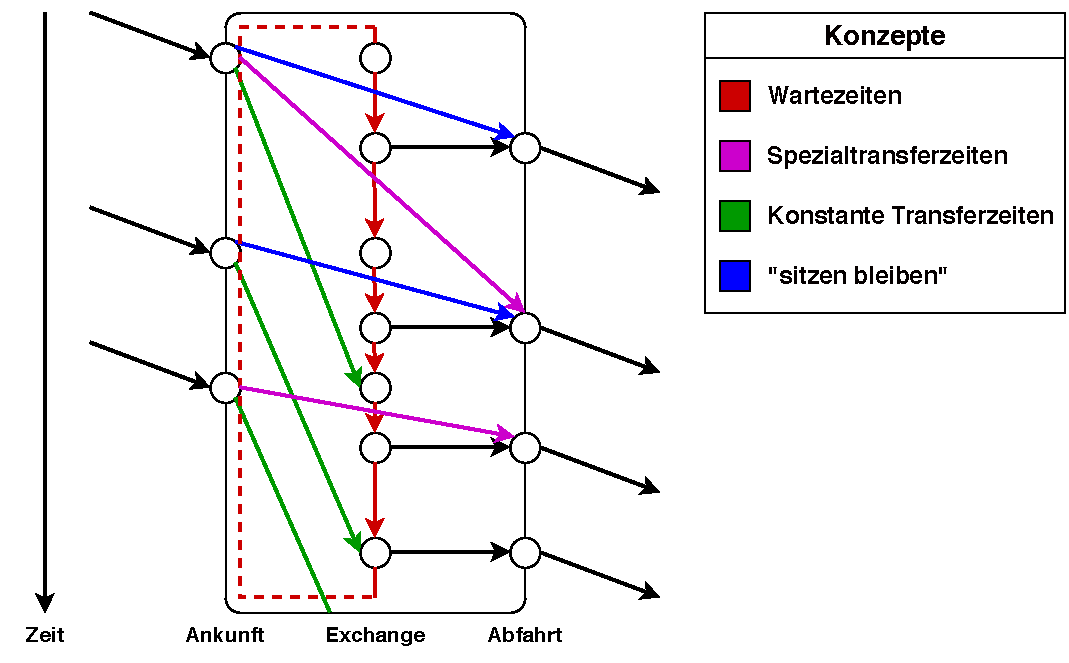
\includegraphics[height=6cm]{images/time-expanded/overview.pdf} 
	\end{center}
\end{frame}